\documentclass{article}
\usepackage{amsmath}
\usepackage{titlesec}
\usepackage[mathletters]{ucs}
\usepackage[utf8x]{inputenc}
\usepackage[margin=1.5in]{geometry}
\usepackage{enumerate}
\newtheorem{theorem}{Theorem}
\usepackage[dvipsnames]{xcolor}
\usepackage{pgfplots}
\pgfplotsset{compat=1.18}
\setlength{\parindent}{0cm}
\usepackage{graphics}
\usepackage{graphicx} % Required for including images
\usepackage{subcaption}
\usepackage{bigintcalc}
\usepackage{pythonhighlight} %for pythonkode \begin{python}   \end{python}
\usepackage{appendix}
\usepackage{arydshln}
\usepackage{physics}
\usepackage{booktabs} 
\usepackage{adjustbox}
\usepackage{mdframed}
\usepackage{relsize}
\usepackage{physics}
\usepackage[thinc]{esdiff}
\usepackage{esint}  %for lukket-linje-integral
\usepackage{xfrac} %for sfrac
\usepackage[colorlinks=true]{hyperref} %for linker, må ha med hypersetup
\usepackage[noabbrev, nameinlink]{cleveref} % to be loaded after hyperref
\usepackage{amssymb} %\mathbb{R} for reelle tall, \mathcal{B} for "matte"-font
\usepackage{listings} %for kode/lstlisting
\usepackage{verbatim}
\usepackage{graphicx,wrapfig,lipsum,caption} %for wrapping av bilder
\usepackage{mathtools} %for \abs{x}
\usepackage[english]{babel}
\usepackage{cancel}
\usepackage{mhchem} % for atom notasjon
\definecolor{codegreen}{rgb}{0,0.6,0}
\definecolor{codegray}{rgb}{0.5,0.5,0.5}
\definecolor{codepurple}{rgb}{0.58,0,0.82}
\definecolor{backcolour}{rgb}{0.95,0.95,0.92}
\lstdefinestyle{mystyle}{
    backgroundcolor=\color{backcolour},   
    commentstyle=\color{codegreen},
    keywordstyle=\color{magenta},
    numberstyle=\tiny\color{codegray},
    stringstyle=\color{codepurple},
    basicstyle=\ttfamily\footnotesize,
    breakatwhitespace=false,         
    breaklines=true,                 
    captionpos=b,                    
    keepspaces=true,                 
    numbers=left,                    
    numbersep=5pt,                  
    showspaces=false,                
    showstringspaces=false,
    showtabs=false,                  
    tabsize=2
}

\lstset{style=mystyle}
\author{Oskar Idland}
\title{Midterm}
\date{}
\begin{document}
\maketitle
%\tableofcontents
\newpage

\section{Cross Sections}
\subsection*{a)}
Number of events observed $W$, cross-section $σ$, integrated luminosity $L$, and the efficiency $ϵ$ are related by the following equation:
\begin{equation}\label{eq: W}
W = σLϵ
\end{equation}
We set $W = 2.25 ⋅ 10^{6}$, $σ = 1$ pb and $ϵ = 0.75$ we can solve for $L$. 
\begin{equation}\label{eq: L}
  L = \frac{W}{σϵ} = 3 ⋅ 10^{6} \text{pb}^{-1} \text{time}^{-1} 
\end{equation}
We do the same for the rare processes:  $W_{r} = 1850$ time$^{-1}$, and background processes: $W_{b} = 1000$ time$^{-1}$. The number of observed rare signal events must therefore be $W_{\text{r,s}} = W_r - W_{b}$, giving $W_{\text{r,s}} = 850$ time$^{-1}$. As the two datasets are equal, their integrated luminosity must be the same, meaning $L_r = L$, which lets us find the cross-section of the rare process. being $σ_r = W_{\text{r,s}} / (Lϵ) = 2.83 ⋅ 10^{-4}$ pb.

\subsection*{b)}
We have the following reactions:
\begin{equation}\label{eq: r_1}
e^{+}e^{-} → μ^{+}μ^{-} γ
\end{equation}
\begin{equation}\label{eq: r_2}
e^{+}e^{-} → q \bar{q}g
\end{equation}
When the electron and anti electron in \cref{eq: r_1} annihilate, they produce a virtual photon if the reaction is through the electromagnetic force. If it is the weak force, then it would be a $Z_0$-boson. The right-hand side is heavier than the left-hand side. This means the electrons would need to have a lot of energy to compensate. If there is energy to spare, the muon might emit a photon as depicted in \cref{fig: 1b1}

\begin{figure}[ht!]
\centering
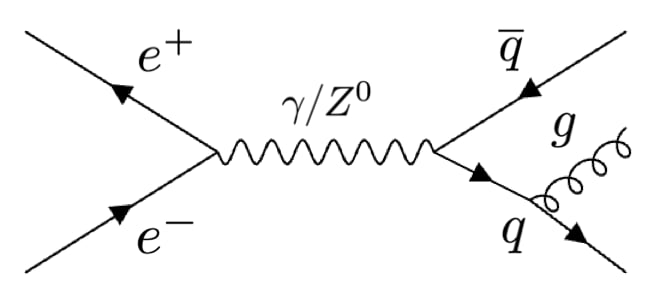
\includegraphics[width = .9\textwidth]{1b1.jpeg}
\caption{Feynman diagram of the process in} \cref{eq: r_1}
\label{fig: 1b1}
\end{figure}


In \cref{eq: r_2}, we again have the electron and anti electron annihilating. The result could be either a virtual photon or a $Z_0$-boson, depending on the force. In this case, it creates a quark and anti-quark, while later emitting a gluon from excess energy, through the strong interaction, as depicted in \cref{fig: 1b2}.
\begin{figure}[ht!]
\centering
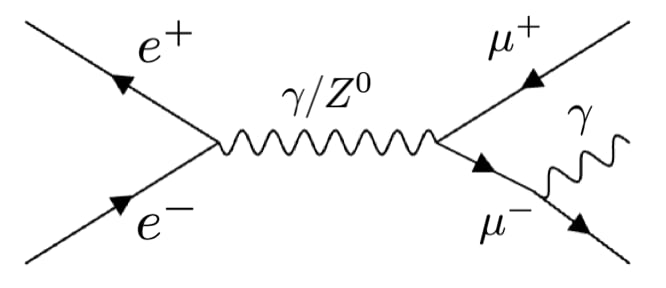
\includegraphics[width = .95\textwidth]{1b2.jpeg}
\caption{Feynman diagram of the process in} \cref{eq: r_2}
\label{fig: 1b2}
\end{figure}

The ratio of the cross-sections of the two reactions is given by the ratio between the fine-structure constant $α$ and the strong coupling constant $α_s$. We get a ratio of $α_s^2 / α^2$



\section{Nuclear Properties and Force}
\subsection*{a)}
\begin{itemize}
    \item \textbf{Rutherford scattering experiment} taught us that the atom is mostly empty space, with a small, dense nucleus carrying the positive charge. This is because the alpha particles, which are positively charged, are deflected by the nucleus, which is also positively charged. Many alpha particles pass through the gold foil without being deflected, which means that the nucleus is very small compared to the atom.
    \item \textbf{Chadwick's scattering experiment} showed that the nucleus also contains neutral particles, named neutrons. This was discovered by bombarding beryllium with alpha particles, which resulted in the emission of neutral radiation.
    \item \textbf{Electron scattering experiments} showed that the nucleus is not a point particle but has a radius which increases with the atomic number $A$ (or mass) which it's charge is distributed over.
    \item \textbf{Hadron scattering experiments} taught us the mass distribution of the nucleus is proportional to the nuclear force and not the Coulomb force.
\end{itemize}


\subsection*{b)}
\textbf{No}, nuclear radius is not a definitive property of the nucleus, as it is not entirely accurate, because the nucleus does not have a well-defined surface. This is shown by electron scattering as the diffraction pattern is not exactly that of a circular disk.


\subsection*{c)}
\begin{enumerate}
    \item \textbf{Charge Independence:} The nuclear force is nearly independent of the charge of the nucleons. We know this from experiments on excited states of \textit{mirror nuclei} like $\ce{_{6}^{11}\text{C}_{5}}$ and $\ce{_{5}^{11}\text{B}_{6}}$. 
    \item \textbf{Attractive and Repulsive:} The nuclear force is strongly attractive distances shorter than 1-2 fm and negligible at greater distances. The nuclear force is repelling at distances shorter than 1 fm. We know the nuclear force is attractive at those smaller distances because of Rutherford scattering experiments. Here we see that the alpha particles needs a certain amount of energy to overcome the Coulomb force and get close enough to the nucleus to be attracted. The linear dependence of the binding energy per nucleon also shows that not all nucleons are attracted by each other at the same time, only the nearest neighbors. 
    \item \textbf{Electrons:} Electrons are not affected by the nuclear force (hence the name)
\end{enumerate}


\section{Nuclear Binding Energy}
\subsection*{a)}
The semi-empirical binding energy formula shows how the binding energy per nucleus depends on the number of electrons and protons as seen in \cref{eq: SEBE}.  When the atoms are small, the nucleons are all close together and therefore the protons are affected by both the nuclear force, and the Coulomb force. When the size of the atom increases, we need more neutrons to keep the nucleus stable, as the extra neutrons provide more attractive nuclear force to counteract the repulsive Coulomb force, and move the protons further apart which again reduces the Coulomb force. This keeps the nucleus stable, but makes the $N / Z$ ration less than one for larger nuclei.   
\begin{equation}\label{eq: SEBE}
B(A,Z) = a_{V}A - a_{S}A^{2/3} - a_{C}\frac{Z(Z-1)}{A^{1/3}} - a_{A}\frac{(A-2Z)^{2}}{A} + \delta(A,Z)
\end{equation}

\subsection*{b)}
There are three components to the semi-empirical binding energy formula as seen in \cref{eq: SEBE}. 
\begin{enumerate}
    \item $\mathbf{a_vA}$: \textbf{Volume term}. The binding energy is proportional to the volume of the nucleus approximated to a sphere $\left(V = 4πR^3/3\right)$. This dominates the binding energy for large nuclei. 
    \begin{equation}
    a_v ≈ 15.8 \text{ MeV}
    \end{equation}
    The linear dependence of the binding energy on the number of nucleons tells us that the strong force is short range as each nucleon only interacts with its nearest neighbors. 
    \item $\mathbf{a_sA^{2 / 3}}$: \textbf{Surface term}. The volume term is not quite accurate as the nucleons on the surface have fewer neighbors. This term corrects for that. The binding energy is proportional to $πR^2$
    \begin{equation}
    a_s ≈ 16.8 \text{ MeV}
    \end{equation} 
    \item $\mathbf{a_cZ(Z-1)A^{-1 / 3}}$: \textbf{Coulomb term}. The binding energy is reduced by the repulsion between the protons. It is therefore detracted. The Coulomb force is long range and is therefore proportional to $Z(Z-1)$ as all protons interact. 
    \begin{equation}
    a_c ≈ 0.72 \text{ MeV}
    \end{equation}
\end{enumerate}

\subsection*{c)}
$\ce{_{}^{16}\text{O}_{}}$ has an even atomic number $A = 16$, and it's number of protons and neutrons are both the magic number $Z = N = 8$. This means that the nucleus is particularly stable.

Between $\ce{_{}^{118}\text{Sn}_{}}$ $\ce{_{}^{119}\text{Sn}_{}}$ we know the latter to have an odd atomic number $A = 119$, making it less stable than the former. We therefore get the list of nuclei in order of stability:

\begin{enumerate}
    \item $\ce{_{}^{16}\text{O}_{}}$
    \item $\ce{_{}^{118}\text{Sn}_{}}$
    \item $\ce{_{}^{119}\text{Sn}_{}}$
\end{enumerate}

\subsection*{d)}
Using an approximation of the $Z_{\text{min}}$ as seen in \cref{eq: Zmin} we get the following for $Z_{\text{min}(136)} = 56.3$ which rounds to the nearest integer $Z_{\text{min}} = 56$. 

Doing the same calculation for $Z_{\text{min}}(135)$ gives $Z_{\text{min}} = 55.97$, which again rounds to the nearest integer $Z_{\text{min}} = 56$. 
\begin{equation}\label{eq: Zmin}
Z_{\text{min}}(A) = \frac{A}{2} \frac{1}{1 + \frac{1}{4}A^{2 / 3}a_c / a_{\text{sym}}} \quad , \quad  a_{\text{syn}} ≈ 23 \text{ MeV} \ , \ a_c ≈ 0.72 \text{ MeV}
\end{equation}

When an even-even nucleus goes through beta decay, it becomes and odd-odd, nucleus. An even-even nucleus will have a higher binding energy, and therefore be more stable. This creates two parabolas for even isobars for when its even-even, and odd-odd, as seen below in figure \ref{fig: mass_parabola}.

\begin{figure}[h!]
\centering
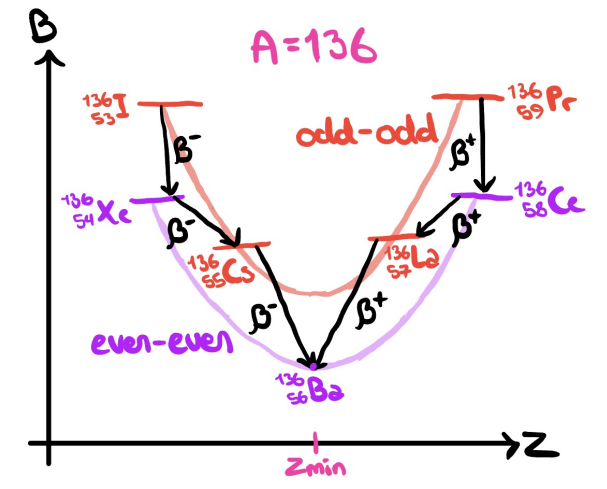
\includegraphics[width = .65\textwidth]{mass_parabola.png}
\caption{Sketch of the mass parabola for $A = 135$, depicting some possible beta decays. The higher up in the graphs, the lower the binding energy.}
\label{fig: mass_parabola}
\end{figure}

In the case of an odd-even nucleus, it will just have a single parabola, as their will always be an extra proton or neutron. 


\section{Nuclear Shell Model}
\subsection*{a)}
There are multiple experimental observations that support the nuclear shell model. The model takes inspiration from the atomic shell model, and the following observations are made:
\begin{enumerate}
    \item \textbf{Magic Numbers:} The magic numbers are the numbers of protons or neutrons that make the nucleus particularly stable. This hints at the existence of shells which are filled with nucleons.
    \item \textbf{Separation Energies:} The separation energies are the energies required to remove a nucleon from the nucleus. The separation energies are not constant, but rather have peaks at the magic numbers. This is because the nucleons in the filled shells are more tightly bound than the nucleons in the unfilled shells.
\end{enumerate}

\subsection*{b)}
\begin{itemize}
    \item The central potential assumes that the nucleons are not interacting with each other, but rather with a central potential. One could use a many-body problem, but this is not practical or always solvable analytically. 
    \item Looking at the nuclear force in a more holistic way makes it easier to calculate how every nucleon interacts with the potential, as a function of radial distance $r$ from the center. 
\end{itemize}

\subsection*{c)}
A common model of the nuclear potential is the Woods-Saxon potential, as seen in \cref{eq: WS}, and illustrated in \cref{fig: WS}. 

\begin{equation}\label{eq: WS}
V(r) = - \frac{V_0}{1 + e^{(r - R)/a}}
\end{equation}
The depth of the potential well is given by $R = R_0 A^{1 / 3}$, as it is the radius of the nucleus. $a$ represent how quickly the potential decreases as $r > R$. It shows both the attractive and repulsive forces in the nucleus. As colored in green, one could add a repulsive component at very close distances to account for the Pauli exclusion principle.

\begin{figure}[h!]
\centering
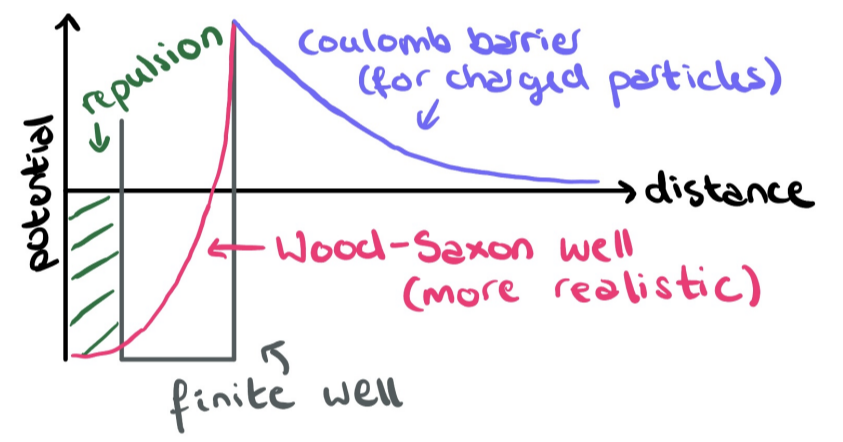
\includegraphics[width = .65\textwidth]{WS.png}
\caption{Illustration of the Woods-Saxon potential.}
\label{fig: WS}
\end{figure}


\subsection*{d)}
We have seven protons and eight neutrons in $\ce{_{}^{15}\text{N}_{}}$. We get the following configuration by filling it's shells. 
\begin{align}
    \text{Proton: } & 1s^{2} \ , \ 1p^{4}_{3 / 2} \ , \ 1p^{1}_{1 / 2} \\
    \text{Neutron: } & 1s^{2} \ , \ 1p^{4}_{3 / 2} \ , \ 1p^{2}_{1 / 2}
\end{align}
The neutrons have all shells filled, and is therefore paired up. The protons have one proton in the $1p_{1 / 2}$ shell, and is therefore unpaired. The proton has angular momentum $l = 1$, giving it parity $π = (-1)^{l} = -1$. Its total angular momentum $J^{π}$ is known to be $1 / 2$ which gives $J^{P} = (1 / 2)^{-}$. 

We can excite the nucleus in multiple ways. 
\begin{enumerate}
    \item Excite a $1p_{1 / 2}$ neutron to $1d_{5 / 2}$.
    \item Excite a $1p_{1 / 2}$ proton to $1p_{1 / 2}$.
    \item Excite a $1p_{3 / 2}$ proton to $1d_{5 / 2}$. Alternatively excite a $1p_{1 / 2}$ proton to $2s_{1 / 2}$, as they are close.
\end{enumerate}
The second and third excitation will be favored as they only leave a single proton unpaired. As there is a smaller energy gap between $1p_{1 / 2}$ and $1d_{5 / 2}$, than from $1p_{3 / 2}$ to $1p_{1 / 2}$, we would expect the first excited state of $\ce{_{}^{15}\text{N}_{}}$ to be the third case. This gives the unpaired proton orbital angular momentum $l = 2$, and parity $π = (-1)^{l} = 1$. This gives the total angular momentum $J^{π}$ to be $(5 / 2)^{+}$.

\subsection*{e)}
We see that the second excited state gives $J^{P} = (1 / 2)^{+}$. This corresponds with option 3 as mentioned above, with the proton in the $2s^{1 / 2}$ orbital, as it has $l = 0$ and $π = 1$. 

The third excited state corresponds with option 2, as we have $J^{P} = (3 / 2)^{-}$. 


\section{Relativistic B-mesoon pairs at SuperKEKB}
\subsection*{a)}
The center of mass energy $\sqrt{s}$ of the colliding electron and anti electron is given by \cref{eq: 5a}.
\begin{equation}\label{eq: 5a}
\sqrt{s} = \sqrt{(E_1 + E_2)^2 - (\vec{p}_1 + \vec{p}_2)^2}
\end{equation}
Expanding the equation gives the following:
\begin{align}
\sqrt{s} &= \sqrt{E_1^2 + E_2^2 + 2E_1E_2 - (\vec{p}_1^2 + \vec{p}_2^2 + 2\vec{p}_1 \cdot \vec{p}_2)c^2} \\
&= \sqrt{m_1^2c^4 + m_2^2c^4 + 2E_1E_2 + m_2^2c^{4} + p_2^2c^{4} - p_1^2c^2 - 2 \cos θp_2p_3c^2 - p_2^2c^2} \\
&= \sqrt{2E_1E_2(1 - \cos θ) + m_1^2c^4 + m_2^2c^4}
\end{align}
$θ$ is the angle between the two colliding particles. A head-on collision would give $θ = π$. Assuming the masses to be approximately zero and adding the energies we get the following:
\begin{equation}
  \sqrt{s} = \sqrt{4 ⋅ 7 \text{ GeV} ⋅  4 \text{ GeV}} = 10.6 \text{ GeV}
\end{equation}

\subsection*{b)}
The following are possible $B$-meson pairs, assuming the top quark lives too short. There are also the anti-particle versions. 
\begin{align}
    B^{+} &: u \bar{b} \\
    B^{+}_c &: c \bar{b} \\
    B^{0} &: d \bar{b} \\
    B^{0}_c &: c \bar{b}
\end{align}
The combined rest energies of the $B$-mesons must be less than the center of mass energy $\sqrt{s}$. The summary table on mesons written by the Particle Data Group (PDG) can be found at \href{https://pdg.lbl.gov/2023/tables/contents_tables.html}{this link}. Here we see that the rest energies from $B^0_{s}$, $B_c^{+}$, $B^{+}$, $B^{0}$ are all less than the center of mass energy, meaning they are the only possible pairs. This goes for their anti-particles as well.

\subsection*{c)}
Relativistic beta and gamma is given by the following:
\begin{align}\label{eq: b_g}
β &= \frac{v}{c} \\
γ &= \frac{1}{\sqrt{1 - β^2}}
\end{align}
If we assume the $B$-mesons to be moving at the same speed, with the same energy, we can input their values from the PDG. Setting their energy as the kinetic energy and assuming energy is conserved, we get the following:
\begin{align}
4E^2_{\text{kin}} + (10.56 \text{ GeV})^2 &= (10.58 \text{ GeV})^2 \\
(5.28 \text{ GeV} / c^2)^2 v^4 &= (10.58 \text{ GeV})^2 - (10.56 \text{ GeV})^2 \\
β^{4} &= \frac{(111.94 - 111.51) \text{ GeV}^2}{27.88 \text{ GeV}^2} \\
β &= 0.35
\end{align}
Now we can find the gamma factor as well. 
\begin{equation}
  γ = \frac{1}{\sqrt{1 - 0.35^2}} = 1.07
\end{equation}


\subsection*{d)}
The average length $L$ the $B$-mesons travel before decay is given by the following:
\begin{equation}
  L = γβcτ 
\end{equation}
Where $τ$ is the proper lifetime of the $B$-mesons. We find its value in the PDG table to be $τ = 1.52 ⋅ 10^{12}$ seconds for the $B^{0}$-meson. This gives us the resulting length:
\begin{equation}
  L = 178 \ μ\text{m}
\end{equation} 



\section{Neutrino Oscillations}
\subsection*{a)}
We know the length of oscillations of two neutrinos $L$ is given by:
\begin{equation}
    L = \frac{4πℏcE_i}{Δm_{ij}^2}
\end{equation}
where $i$ and $j$ can have values 1,2 and 3 for the different generations. We use natural units where $ℏ = c = 1$. This is related to the probability of finding a neutrino of generation $j$ at distance $L$ as the following:
\begin{equation}
  P(ν_i → ν_j) = \sin ^2(2θ_{ij}) \sin ^2(L / L_0)
\end{equation}
Setting $i = 2$ and $j = 1$, we can calculate the distance of maximum intensity of electron neutrinos. First we get the energie of the muon neutrino $E_2 = 0.1$ GeV, with the mass difference $Δm_{21}^2 = 7.5 ⋅ 10^{-23}$ GeV. Now we can calculate the length $L_0$:
\begin{equation}
  L_0 = 5.3 ⋅ 10^{21} \text{ GeV}^{-1} = 1.1 ⋅ 10^{6} \text{ m}
\end{equation}
This is using the fact in natural units, $1$ GeV$^{-1}$$ = 0.197 ⋅ 10^{-15}$ m. 

The first peak of probability is found at $L / L_0 = π / 2$. This allows us to find the first length with peak intensity of electron neutrinos.
\begin{equation}
  L_{\text{max}} = 1.7 ⋅ 10^{6} \text{ m}
\end{equation} 

\subsection*{b)}
If we insert the distance found in the previous task in our equation of probability we get the following:
\begin{equation}
  P(ν_{μ} → ν_{e}) = \sin ^2 (2 \arctan \sqrt{0.444}) = 0.85
\end{equation}
This can be flipped to find the probability of muon neutrinos at the same distance.
\begin{equation}
  P(ν_{e} → ν_{μ}) = 1 - P(ν_{μ} → ν_{e}) = 0.15
\end{equation}
This means the relative intensity of muon neutrinos is $15 \%$ and electron neutrinos $85 \%$ at the distance $L_{\text{max}}$.


\section{Quantum Numbers}
\subsection*{a)}
As $^{1}S_0$ is a singlet state it will have $J = 0$ with spin and  orbital angular momentum $S = L = 0$. The P-parity is therefore $(-1)^{L + 1} = -1$. The C-parity is therefore $(-1)^{L + S} = 1$. In conclusion we get $J^{PC} = 0^{-+}$. The quantum numbers used do not depend on particle type, just spin and angular momentum, so the result would be the same for the same state of bound $e^{+}e^{-}$.  

\subsection*{b)}
\textbf{No}. The same bound state of $b\bar{b}$ can not be produced directly by collisions of $e^{+}e^{-}$, because the initial state of the latter is not a $^{1}S_0$ bound state. This is caused by the need to obey Fermi statistics, which requires the wave function to be antisymmetric under exchange of the two particles. When annihilating, we find the particles at the same location, which means a symmetric wave spacial function. The spin part is also symmetric so the total wave function is symmetric. 

\subsection*{c)}
Only $π^{0}$ is an eigenstate of C-parity. This is because if you flip the charge, you still have the same particle (aka. quantum state). Flipping the charge of $π^{+}$ gives $π^{-}$, and flipping the charge of $π^{-}$ gives $π^{+}$, which are different particles and therefore not an eigenstate. 


\section{Allowed, Suppressed and Forbidden Processes}
\subsection*{a)}
\begin{equation}\label{eq: s_1}
ν_ee^{-} → ν_{μ}μ^{-}
\end{equation}
\cref{eq: s_1} will be evaluated on the following:
\begin{itemize}
    \item \textbf{Lepton Number:} The number of leptons of each generation is not conserved.  
    \item \textbf{Baryon Number:} The number of baryons is conserved as there are no baryons on either side.
    \item \textbf{Charge:} The charge is conserved going from $-1$ to $-1$. 
    \item \textbf{Mass:} The mass is increases as the left-hand side is much lighter than the right-hand side due to the massive muon. 
\end{itemize}
The process in \cref{eq: s_1} is \textbf{forbidden} because the lepton number of each generation is not conserved. 

\subsection*{b)}
\begin{equation}\label{eq: s_2}
Λ^{0} → p^{+} π^{-}
\end{equation}
\cref{eq: s_2} will be evaluated on the following:
\begin{itemize}
    \item \textbf{Lepton Number:} There are no leptons on either side, so the lepton number is conserved.
    \item \textbf{Baryon Number:} There is one baryon on the left-hand side and one on the right-hand side (the proton). The baryon number is conserved.
    \item \textbf{Charge:} The charge is conserved going from 0 tone net charge of $+1 -1 = 0$.
    \item \textbf{Mass:} The mass decreases as $Λ^{0}$ is much heavier than the proton and the pion.
\end{itemize}
The process in \cref{eq: s_2} is \textbf{allowed} because the mass is decreased and the other conservation laws are conserved. The process is mediated by the weak force as depicted in \cref{fig: 8b}, where the strange quark in the $Λ^{0}$ decays into a up quark and emits a $W^{-}$ boson which turns into a $π^{-}$. 
 
\begin{figure}[ht!]
\centering
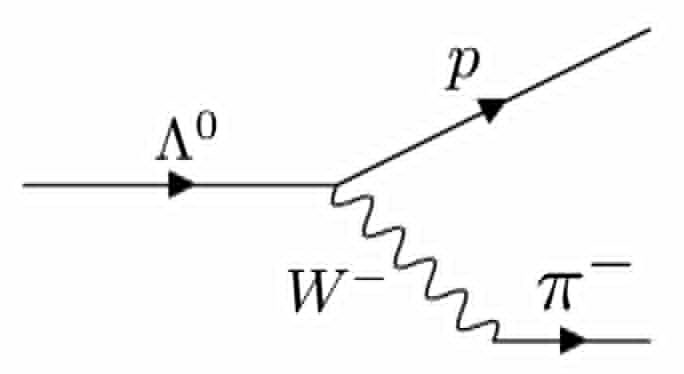
\includegraphics[width = .45\textwidth]{8b.jpeg}
\caption{Feynman diagram of the process in} \cref{eq: s_2}
\label{fig: 8b}
\end{figure}

\subsection*{c)}
\begin{equation}\label{eq: s_3}
μ^{+}μ^{-} →  t\bar{t} 
\end{equation}
\cref{eq: s_3} will be evaluated on the following:
\begin{itemize}
    \item \textbf{Lepton Number:} The number of leptons is conserved going from net 0 to 0.
    \item \textbf{Baryon Number:} The number of baryons is conserved going from 0 to 0.
    \item \textbf{Charge:} The charge is conserved going from $-1 + 1 = 0$ to $2 / 3 - 2 / 3 = 0$.
    \item \textbf{Mass:} The mass increases from the left-hand side to the right-hand side.
\end{itemize}
The process in \cref{eq: s_3} is \textbf{suppressed} because the mass is increased. It would most likely be mediated by the weak interaction, but potentially also the electromagnetic force, as depicted in \cref{fig: 8c}.

\begin{figure}[ht!]
\centering
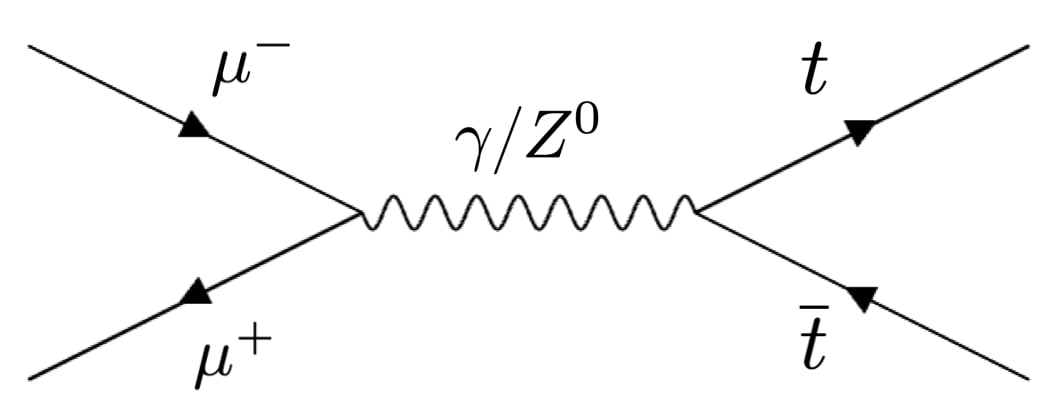
\includegraphics[width = .45\textwidth]{8c.jpeg}
\caption{Feynman diagram of the process in} \cref{eq: s_3}
\label{fig: 8c}
\end{figure}


\subsection*{d)}
\begin{equation}\label{eq: s_4}
\bar{p} → ne^{-}\bar{ν}_e
\end{equation}
\cref{eq: s_4} will be evaluated on the following:
\begin{itemize}
    \item \textbf{Lepton Number:} The number of leptons is conserved going from 0 to net 0.
    \item \textbf{Baryon Number:} The number of baryons is not conserved going from $-1$ to $1$.
    \item \textbf{Charge:} The charge is conserved going from $-1$ to $-1$.
    \item \textbf{Mass:} The mass decreases from the left-hand side to the right-hand side.
\end{itemize}
The process in \cref{eq: s_4} is \textbf{forbidden} because the baryon number is not conserved. 
\end{document}

